\documentclass[]{beamer}
\usepackage[T1]{fontenc}
\usepackage[utf8]{inputenc}
\usepackage{lmodern}
\usepackage[italian]{babel}
\usepackage{mathrsfs}

\title{Le equazioni di Maxwell e le onde elettromagnetiche}
\author{\texorpdfstring{Mattia Cozzi\newline\href{mailto:cozzimattia@gmail.com}{\texttt{cozzimattia@gmail.com}}}{Mattia Cozzi}}
\date{a.s.~2023/2024}

%\documentclass[handout]{beamer}     %usare questa classe per generare l'handout
%\usepackage{pgfpages}   %per mostrare più quadri nella stessa pagina
%\pgfpagesuselayout{4 on 1}[a4paper,border shrink=5mm,landscape]
\usetheme{Singapore}
%\useoutertheme[left]{sidebar} %elementi intorno alle diapositive
\setbeamercovered{dynamic} %modifica l'aspetto del testo grigetto delle diapositive future. Argomenti: invisible/transparent/dynamic
\usecolortheme{orchid}
%COLORE PRINCIPALE
\definecolor{marroncino}{RGB}{156, 26, 0} % UBC Blue (primary)
\setbeamercolor{structure}{fg=marroncino} % itemize, enumerate, etc

\theoremstyle{plain}
\newtheorem{teorema}{Teorema}

\usepackage{tikz}
\usepackage{circuitikz}

\usepackage{pgf,pgfplots,graphicx}
\usetikzlibrary{angles,quotes,arrows,shapes,decorations.markings}
\pgfplotsset{compat=1.15}
\usepgfplotslibrary{units,fillbetween} % to add units easily to axis

\newcommand{\fem}{f_{em}}

\def\angolo[#1](#2)(#3:#4:#5)% Syntax: [draw options] (center) (initial angle:final angle:radius)
    { \draw[#1] ($(#2)+({#5*cos(#3)},{#5*sin(#3)})$) arc (#3:#4:#5); }


\begin{document}

\begin{frame}
  \titlepage
\end{frame}





\begin{frame}
\frametitle{Contenuti}
\tableofcontents
\end{frame}


\section{Equazioni}

\begin{frame}
\frametitle{James Clerk Maxwell}
\begin{columns}
\begin{column}{0.2\textwidth}
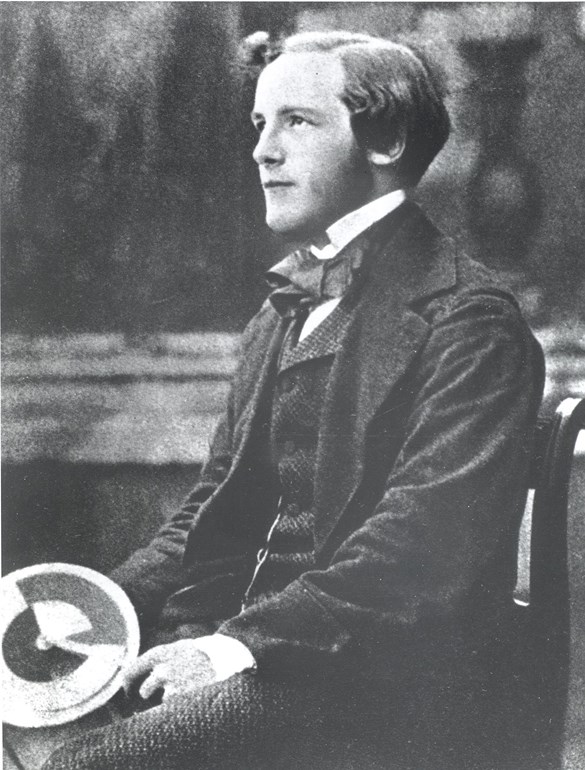
\includegraphics[width=\columnwidth]{img/maxwell.jpg}
\end{column}
\begin{column}{0.7\textwidth}
\begin{itemize}
\item<1-> 1861: James Clerk Maxwell pubblica \emph{On Physical Lines of Force};
\item<2-> 1873: Maxwell pubblica \emph{Treatise On Electricity and Magnetism}, in cui dimostra che \alert<2>{tutte le proprietà elettriche, magnetiche e induttive possono essere derivate da sole quattro equazioni}, che fungono da \alert<2>{assiomi} della teoria;
\item<3-> Maxwell struttura e amplia il discorso fatto dai fisici precedenti sui fenomeni elettrici e magnetici.
\end{itemize}
\end{column}
\end{columns}
\end{frame}


\begin{frame}
\frametitle{Le equazioni di Maxwell (caso generale)}
  Le \alert{equazioni di Maxwell} per il caso generale sono:\begin{enumerate}
  \item Teorema di Gauss per il campo elettrico
  \begin{center}
  \colorbox{marroncino!30}{$ \Phi_S (\vec{E}) = \dfrac{Q_{tot}}{\varepsilon_0} $}
  \end{center}\pause
  \item Teorema di Gauss per il campo magnetico
  \begin{center}
  \colorbox{marroncino!30}{$ \Phi_S (\vec{B}) = 0 $}
  \end{center}\pause
  \item Legge di Faraday-Neumann-Lenz
  \begin{center}
\colorbox{marroncino!30}{  $ \Gamma_\mathscr{L} (\vec{E}) = -\dfrac{d\Phi_S(\vec{B})}{dt} $}
  \end{center}\pause
  \item Teorema di Ampère-Maxwell
  \begin{center}
  \colorbox{marroncino!30}{$ \Gamma_\mathscr{L} (\vec{B}) = \mu_0 \left( i + \varepsilon_0 \dfrac{d\Phi_S(\vec{E})}{dt} \right) $}
  \end{center}
\end{enumerate}
\end{frame}



\begin{frame}
  \frametitle{1.~Il teorema di Gauss per $ \vec{E} $}
    \begin{center}
  \colorbox{marroncino!30}{$ \Phi_S (\vec{E}) = \dfrac{Q_{tot}}{\varepsilon_0} $}
  \end{center}\pause
  Dice che:
  \begin{itemize}
    \item le linee del campo elettrico possono essere aperte;\pause
    \item esistono cariche elettriche isolate;\pause
    \item le cariche sono le sorgenti del campo elettrico.
  \end{itemize}
\end{frame}

\begin{frame}
  \frametitle{2.~Il teorema di Gauss per $ \vec{B} $}
    \begin{center}
  \colorbox{marroncino!30}{$ \Phi_S (\vec{B}) = 0 $}
  \end{center}\pause
  Dice che:
  \begin{itemize}
    \item per ogni linea di campo entrante c'è una linea di campo uscente, ovvero tutte le linee del campo magnetico sono chiuse;\pause
    \item non esistono poli magnetici isolati.
  \end{itemize}
\end{frame}

\begin{frame}
  \frametitle{3.~La legge di Faraday-Neumann-Lenz}
  \begin{center}
\colorbox{marroncino!30}{  $ \Gamma_\mathscr{L} (\vec{E}) = -\dfrac{d\Phi_S(\vec{B})}{dt} $}
  \end{center}\pause
  Dice che:
  \begin{itemize}
    \item un campo magnetico variabile è sorgente di un campo elettrico.\pause
    \item il campo elettrico è conservativo solo se è statico.
  \end{itemize}
\end{frame}

\begin{frame}
  \frametitle{4.~Il teorema di Ampère-Maxwell}
  \begin{center}
\colorbox{marroncino!30}{$ \Gamma_\mathscr{L} (\vec{B}) = \mu_0 \left( i + \varepsilon_0 \dfrac{d\Phi_S(\vec{E})}{dt} \right) $}
  \end{center}\pause
  Dice che:
  \begin{itemize}
    \item il campo magnetico non è conservativo;\pause
    \item le cariche in moto (le correnti) e i campi elettrici variabili sono le sorgenti del campo magnetico.
  \end{itemize}
\end{frame}


\section{Onde}

\begin{frame}
  \frametitle{Il campo elettromagnetico}
Nelle ultime due equazioni \alert<1>{compaiono sia $ \vec{E} $ sia $ \vec{B} $}:{\pause} non è più possibile studiare i due campi separatamente; essi risultano essere \alert<2>{due aspetti di un unico fenomeno}:\pause

~

\begin{block}{Campo elettromagnetico}
Il campo elettrostatico e il campo magnetico sono solo casi particolari del campo elettromagnetico; si ottengono, rispettivamente, soltanto se si hanno cariche ferme oppure correnti continue.
\end{block}
\end{frame}






\begin{frame}
  \frametitle{Propagazione dei campi}
  Se facciamo oscillare una carica in una certa zona dello spazio (ad esempio mediante una \emph{corrente alternata}) otteniamo un \alert<1>{campo elettrico variabile},{\pause} che genera un \alert<2>{campo magnetico variabile},{\pause} che induce un \alert<3>{campo elettrico variabile},{\pause} che genera un \alert<4>{campo magnetico variabile}, ecc.\\\pause~\\Ciò che si ottiene è un'\alert<5>{onda elettromagnetica}, una propagazione ondulatoria del campo elettromagnetico.
\end{frame}



\begin{frame}
  \frametitle{Onde elettromagnetiche}
  Le onde elettromagnetiche:
  \begin{itemize}
    \item furono previste da Maxwell nel 1861 a partire dalle sue equazioni differenziali e dimostrate sperimentalmente da Heinrich Rudolph Hertz nel 1889;\pause
    \item non richiedono un mezzo materiale e si propagano anche nel vuoto;\pause
    \item si muovono nel vuoto a velocità:
    \begin{center}
    $ c = \dfrac{1}{\sqrt{\varepsilon_0 \mu_0}} = 2,998 \times 10^8 \, \frac{m}{s} $
    \end{center}
    e hanno come caso particolare la luce.
  \end{itemize}
\end{frame}


\begin{frame}
  \frametitle{Profilo spaziale delle onde}
  Nelle onde elettromagnetiche i valori oscillanti dei due campi sono legati dalla relazione:
  \begin{center}
  $ E = cB $
  \end{center}
  ed essi oscillano su \emph{piani perpendicolari} tra loro e alla direzione di propagazione dell'onda.\pause
  \begin{figure}
    \begin{tikzpicture}[x={(-10:1cm)},y={(90:1cm)},z={(210:1cm)},scale=.8]
    % Axes
    \draw (-1,0,0) node[above] {$x$} -- (5,0,0);
    \draw (0,0,0) -- (0,2,0) node[above] {$y$};
    \draw (0,0,0) -- (0,0,2) node[left] {$z$};
    % Propagation
    \draw[->, thick] (5,0,0) -- node[above] {$c$} (6,0,0);
    % Waves
    \draw[red,thick] plot[domain=0:4.5,samples=200] (\x,{cos(deg(pi*\x))},0);
    \draw[blue,thick] plot[domain=0:4.5,samples=200] (\x,0,{cos(deg(pi*\x))});
    % Arrows
    \foreach \x in {0.1,0.3,...,4.4} {
      \draw[->,help lines] (\x,0,0) -- (\x,{cos(deg(pi*\x))},0);
      \draw[->,help lines] (\x,0,0) -- (\x,0,{cos(deg(pi*\x))});
    }
    % Labels
    \node[above right] at (0,1,0) {$\vec{E}$};
    \node[below] at (0,0,1) {$\vec{B}$};
  \end{tikzpicture}
  \end{figure}
\end{frame}

\begin{frame}
  \frametitle{Frequenza e lunghezza d'onda}
  Essendo la velocità dell'onda costante, la frequenza delle oscillazioni e la lunghezza d'onda sono inversamente proporzionali secondo la relazione:
   \begin{center}
   \colorbox{marroncino!30}{$ f = \dfrac{c}{\lambda} $}
   \end{center}
\end{frame}


\section{Spettro}

\begin{frame}
\frametitle{Frequenze e lunghezze d'onda diverse}
  Ciò che distingue un'onda elettromagnetica da un'altra è la sua frequenza (e di conseguenza la sua lunghezza d'onda).\\\pause~\\
  \begin{block}{Spettro elettromagnetico}
    Lo spettro elettromagnetico è l'insieme delle frequenze delle onde elettromagnetiche.
  \end{block}\pause
  
  ~
  
  In particolare, la \alert{luce visibile} è un'onda elettromagnetica con lunghezza d'onda tra $ 7 \times 10^{-7} \, m = 700 \, nm $ (rosso) e $ 4 \times 10^{-7} \, m = 400 \, nm $ (violetto).
\end{frame}


\begin{frame}
\frametitle{Lo spettro elettromagnetico}
  \begin{figure}
  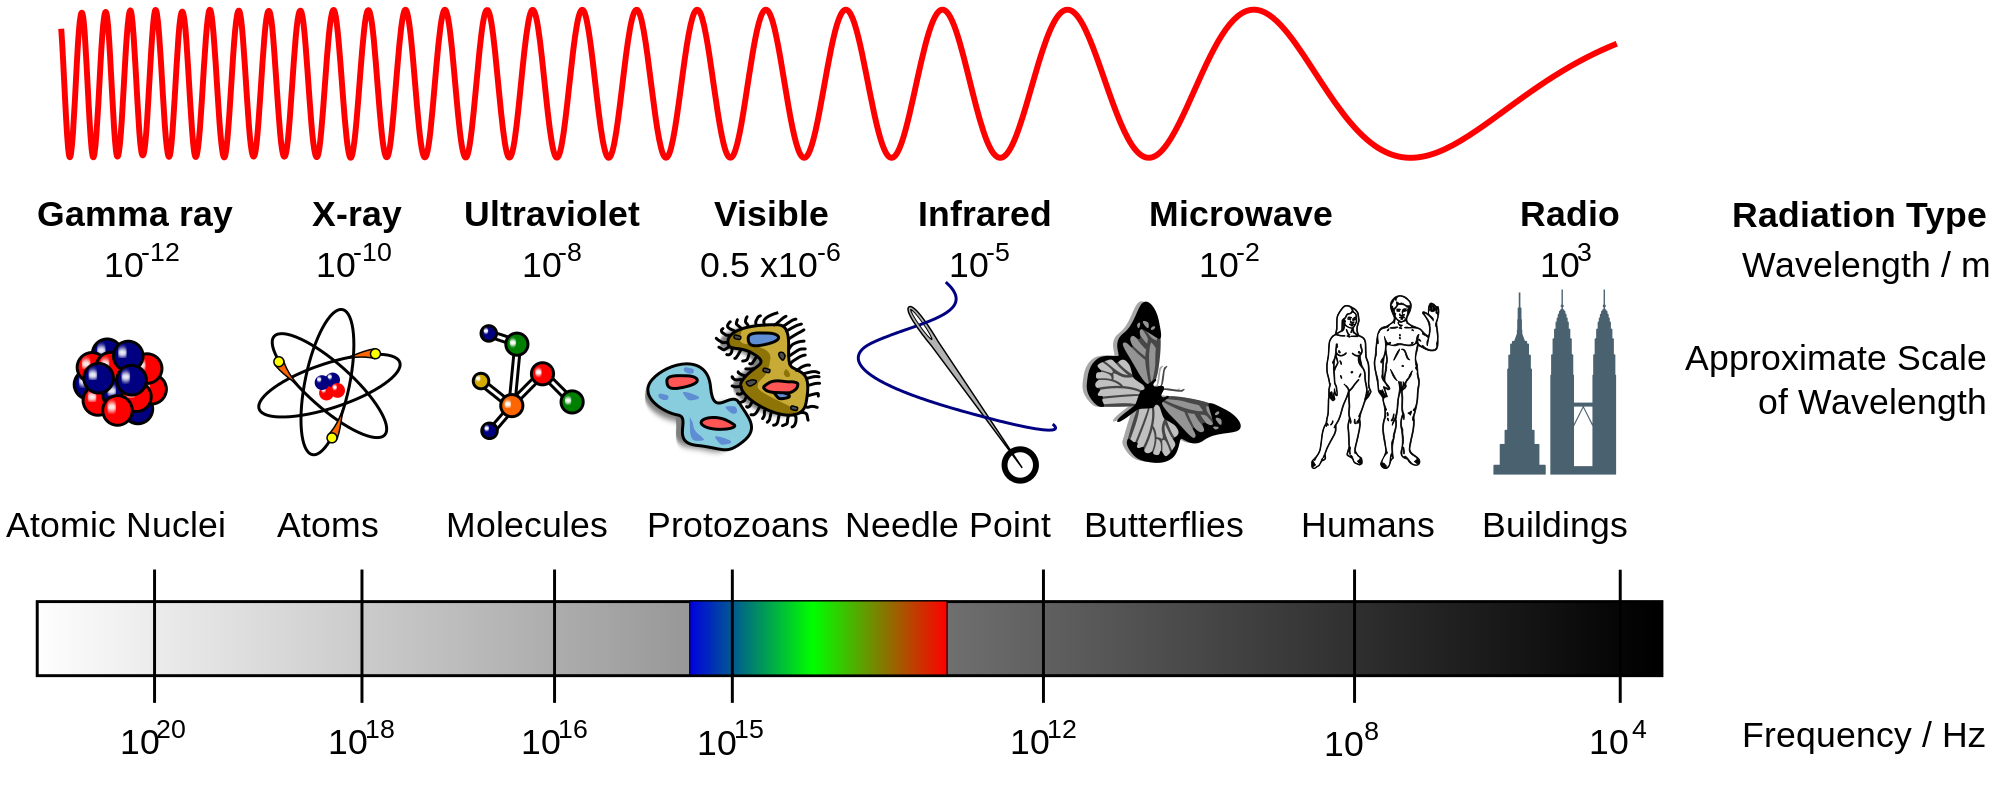
\includegraphics[width=\columnwidth]{img/spettroem.png}
  \end{figure}
\end{frame}



\begin{frame}
\frametitle{Tipi di onde (1)}
  \begin{columns}
    \begin{column}{0.3\textwidth}
      \begin{figure}
        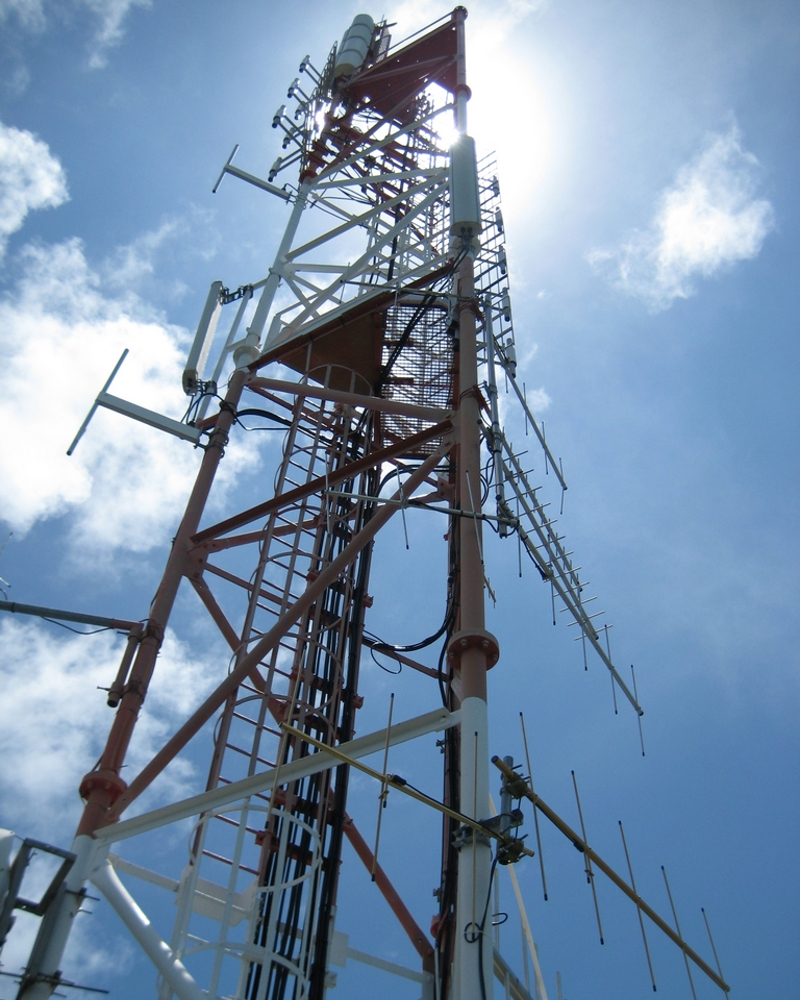
\includegraphics[width=.7\columnwidth]{img/radio.jpg}
      \end{figure}
      \begin{footnotesize}
      \textbf{Onde radio:} $ 10 \, km - 10 \, cm $\\
      Le onde più lunghe di $ 10 \, m $ sono riflesse dalla ionosfera e possono superare la curvatura terrestre.
      \end{footnotesize}
    \end{column}
    \begin{column}{0.3\textwidth}
      \visible<2-3>{\begin{figure}
        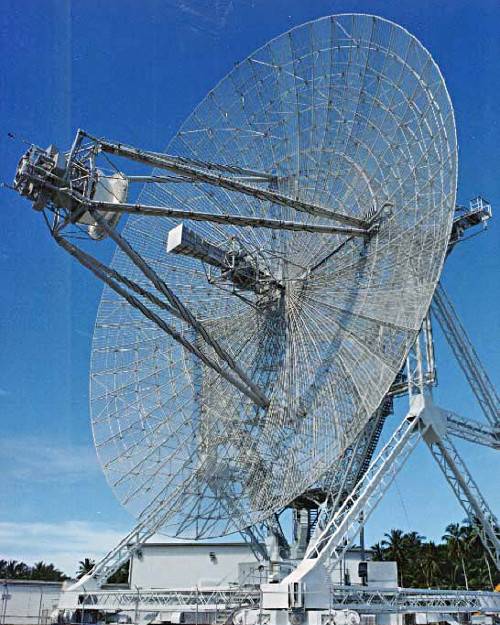
\includegraphics[width=.7\columnwidth]{img/micro.jpg}
      \end{figure}
      \begin{footnotesize}
      \textbf{Microonde:} $ 10 \, cm - 1 \, mm $\\
      Sono usate da cellulari GSM, dai radar, nella comunicazione coi satelliti e nei forni a microonde.
      \end{footnotesize}}
    \end{column}
    \begin{column}{0.3\textwidth}
      \visible<3>{\begin{figure}
        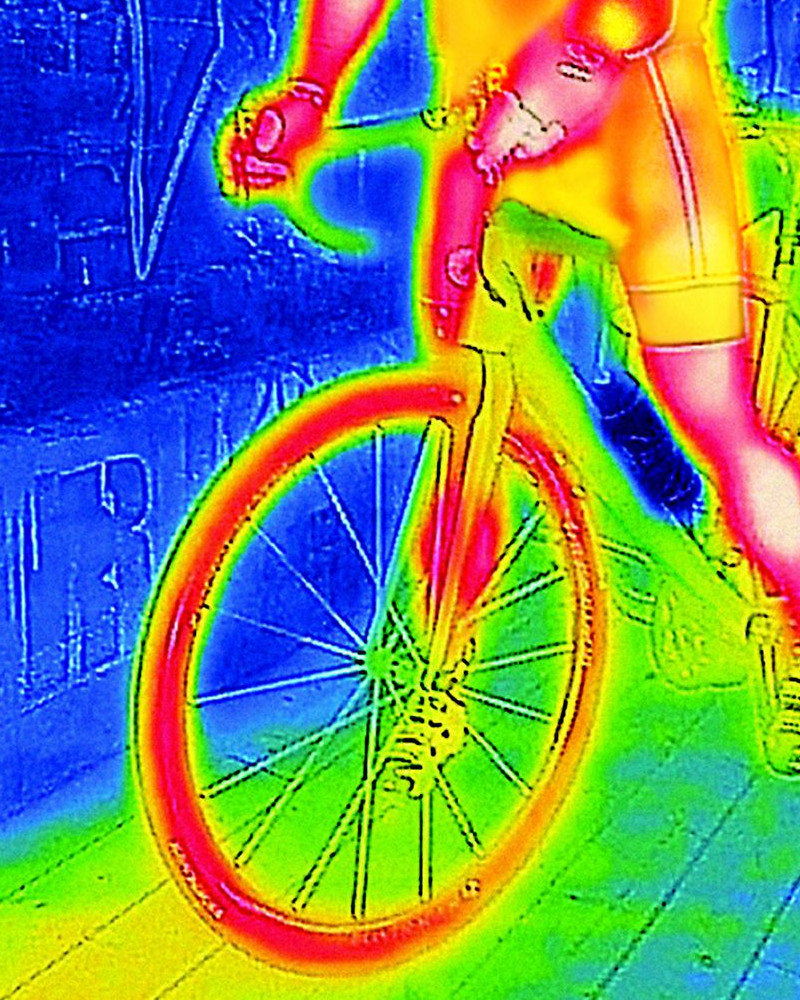
\includegraphics[width=.7\columnwidth]{img/ir.jpg}
      \end{figure}
      \begin{footnotesize}
      \textbf{Radiazione infrarossa:} $ 1 \, mm - 7 \times 10^{-7} \, m $\\
      La percepiamo  come calore ed è usata per la termografia, per la visione notturna e nei telecomandi.
      \end{footnotesize}}
    \end{column}

  \end{columns}
\end{frame}


\begin{frame}
\frametitle{Tipi di onde (2)}
  \begin{columns}
    \begin{column}{0.3\textwidth}
      \begin{figure}
        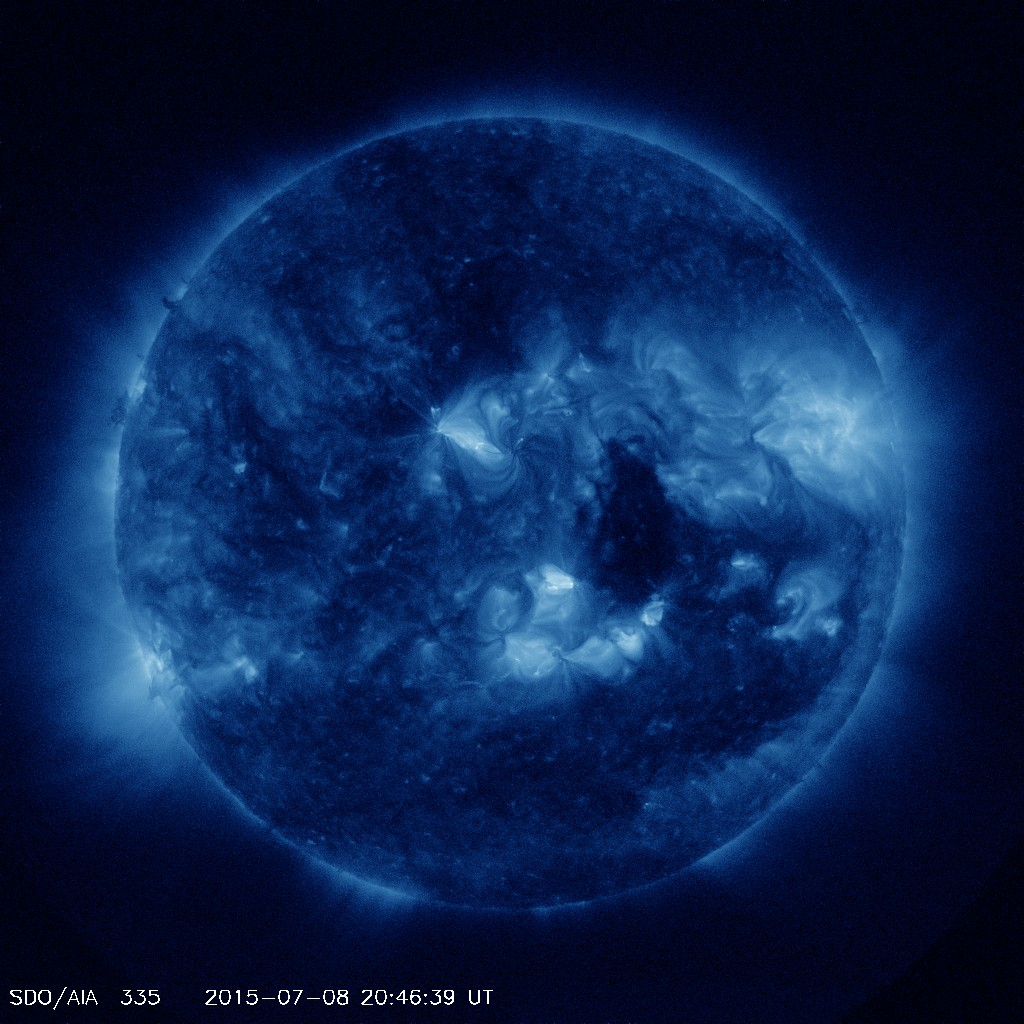
\includegraphics[width=.8\columnwidth]{img/uv.jpg}
      \end{figure}
      \begin{footnotesize}
      \textbf{Raggi ultravioletti:} $ 4 \times 10^{-7} \, m - 1 \times 10^{-8} \, m $\\
      Favoriscono la produzione di melanina nel corpo (non esagerare!) e sono usati in astronomia.
      \end{footnotesize}
    \end{column}
    \begin{column}{0.3\textwidth}
      \visible<2-3>{\begin{figure}
        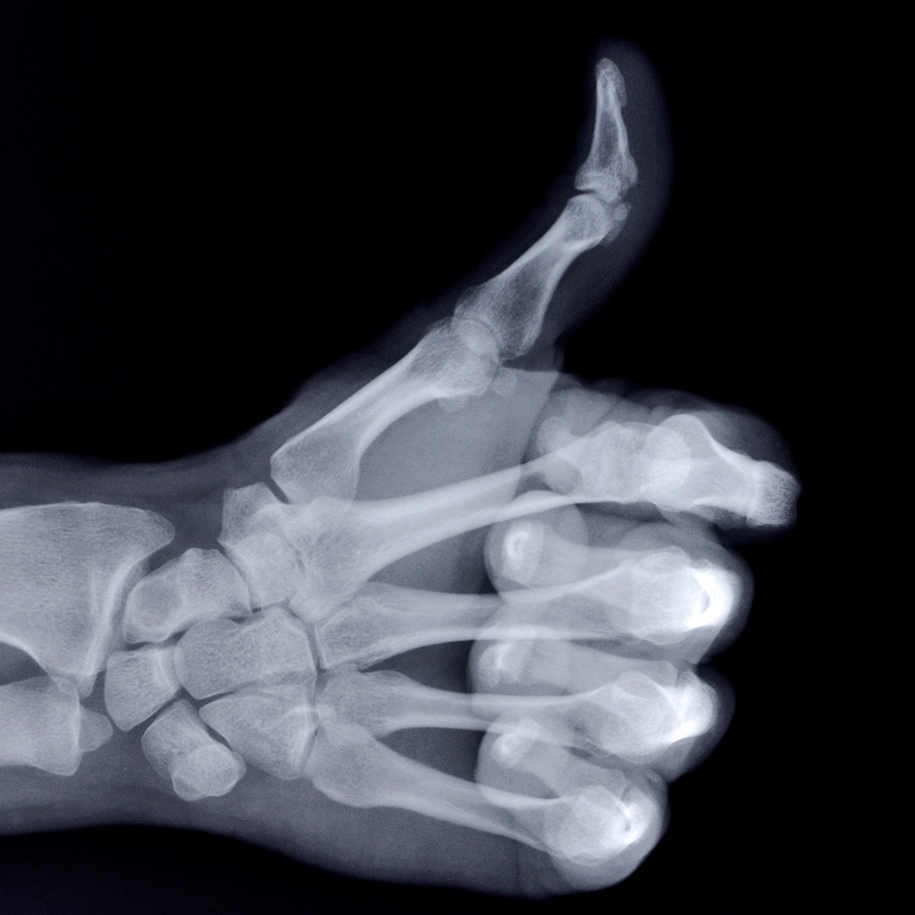
\includegraphics[width=.8\columnwidth]{img/x.jpg}
      \end{figure}
      \begin{footnotesize}
      \textbf{Raggi X:} $ 1 \times 10^{-8} \, m - 1 \times 10^{-11} \, m $\\
      Attraversano i tessuti molli del corpo, ma sono arrestati dalle ossa, usati per le radiografie.
      \end{footnotesize}}
    \end{column}
    \begin{column}{0.3\textwidth}
      \visible<3>{\begin{figure}
        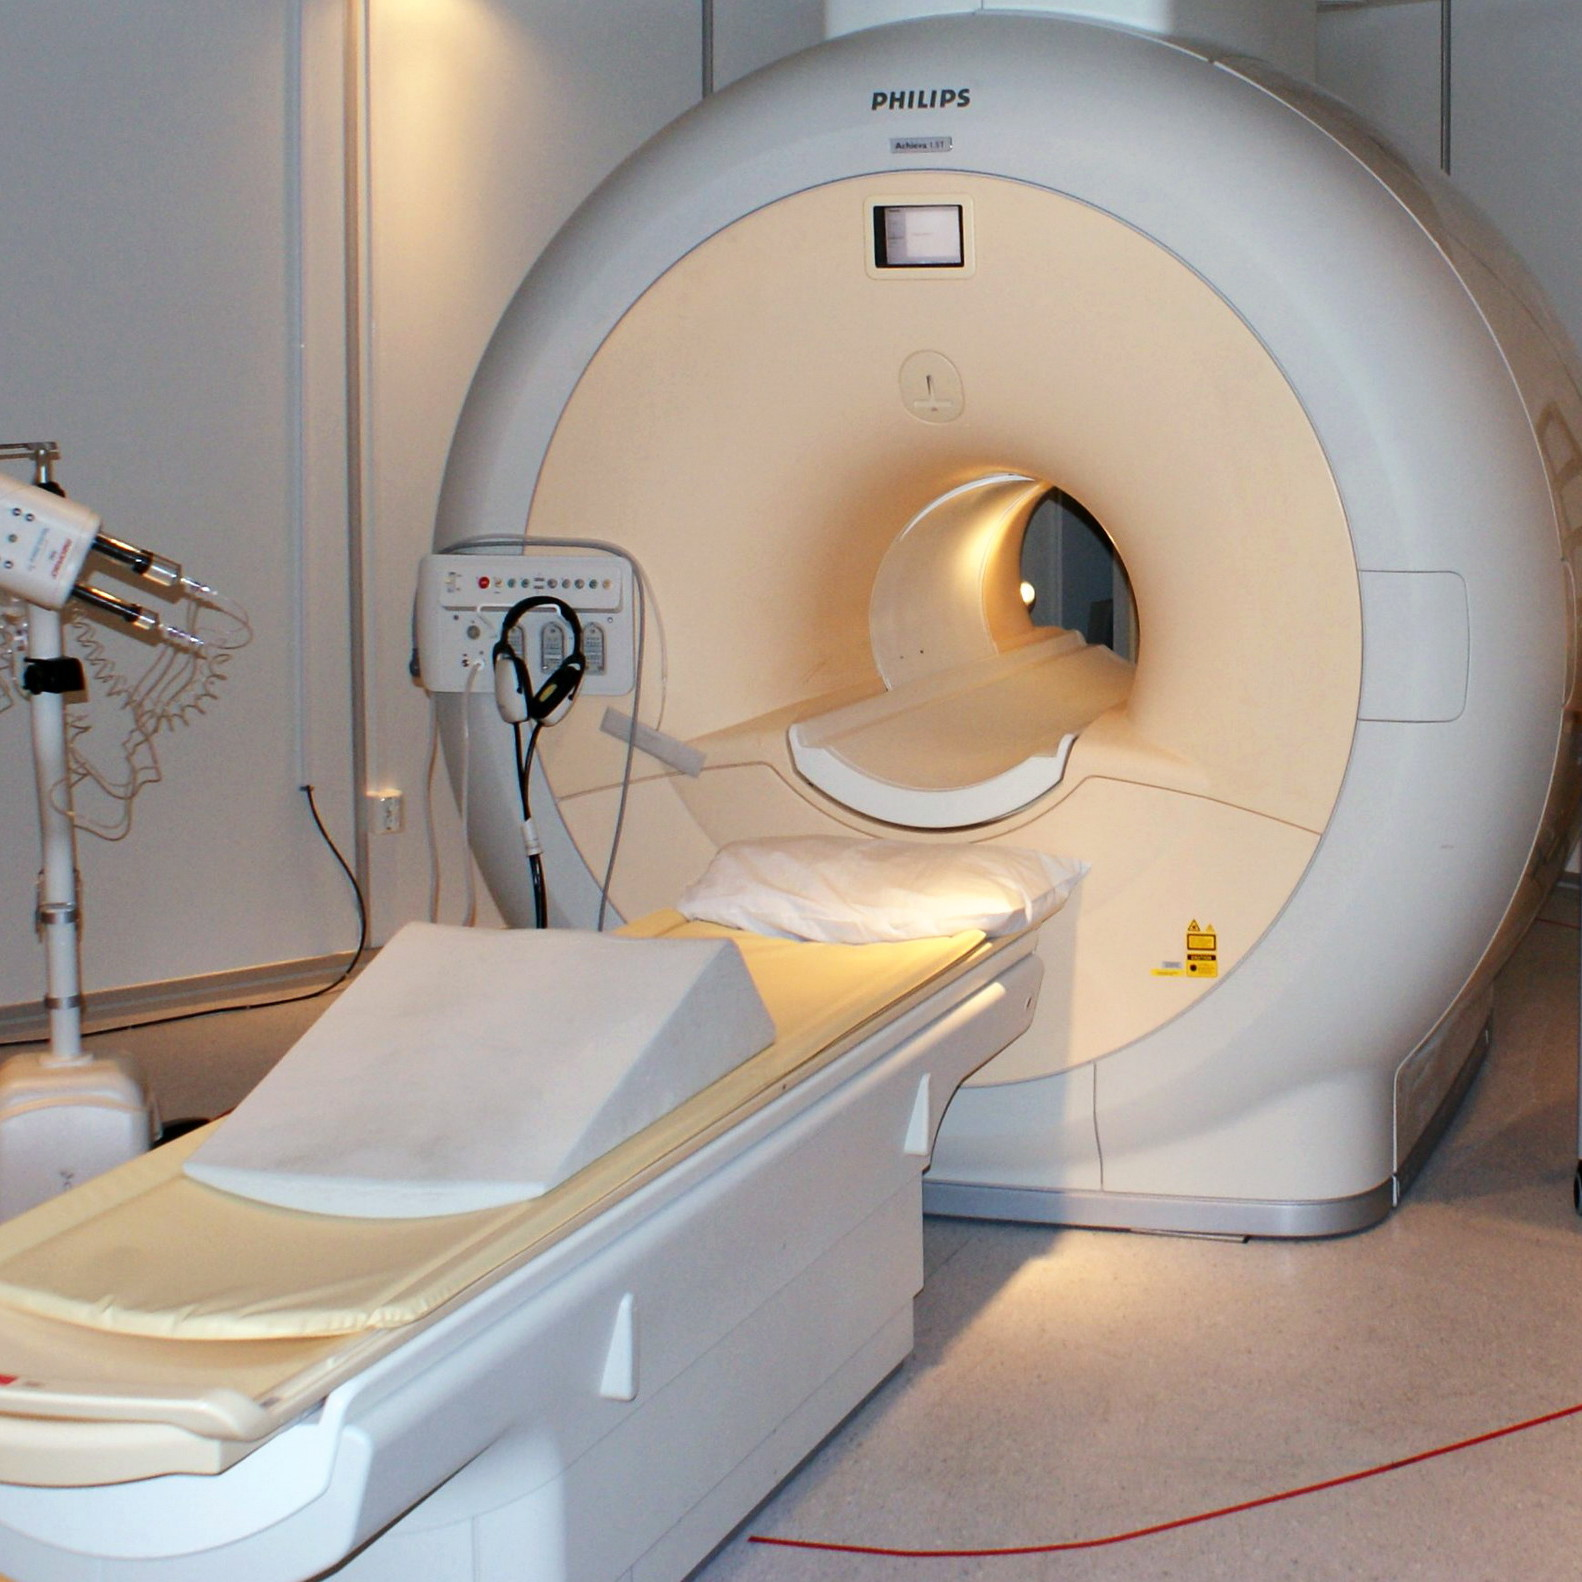
\includegraphics[width=.8\columnwidth]{img/gamma.jpg}
      \end{figure}
      \begin{footnotesize}
      \textbf{Raggi gamma:} $ < 1 \times 10^{-12} \, m $\\
      Accompagnano fenomeni di radioattività e reazioni nucleari, utilizzati in radioterapia.
      \end{footnotesize}}
    \end{column}

  \end{columns}
\end{frame}

%sezione su polarizzazione ecc

%
% \section{Problemi}
%
% \begin{frame}
% Osservazioni generali sulle equazioni, chiudono il cerchio
%
% problema dell'invarianza di c
% \end{frame}
%

\end{document}
